%!TEX root = paper.tex


\section{Fault Tolerance via Asynchronous Snapshots}
\label{sec:snapshots}
Fault tolerance in Flink is achieved by taking a snapshot of the execution graph at regular intervals. When failure occurs the state of the execution is restored from the latest snapshot. Upon recovery, in order to guarantee exactly-once processing semantics, the records (events) consumed since the dryad snapshot are reprocessed in the same order at each respective source. Normally this possible by using persistent message queueing systems, e.g. Apache Kafka.

\begin{figure}[ht]
	\centering  	
  	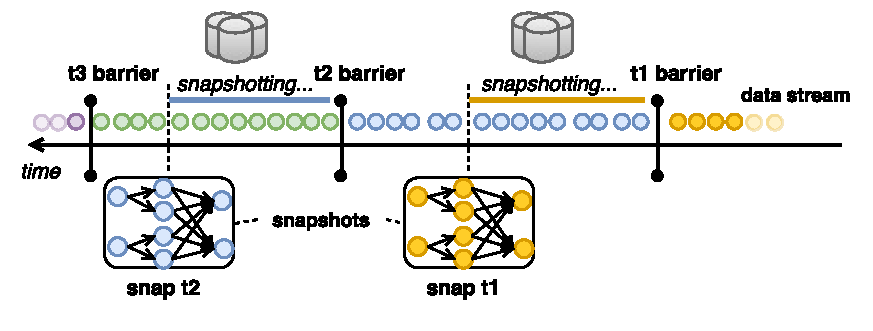
\includegraphics[width=.75\textwidth]{figs/snaps.pdf}
  	\vspace{-4mm}
	\caption{Asynchronous Barrier Snapshotting.}
	\vspace{-2mm}
	\label{fig:FlinkStack}
\end{figure}

Flink's core mechanism for distributed snapshots is called ``Asynchronous Barrier Snapshotting'' (ABS).~\cite{carbone2015lightweight} It creates a global snapshot by collecting the state of each task in the execution graph in an asynchronous manner. It does so by superimposing snapshotting using injected markers, called ``barriers'', in the input data stream. Similar to Chandy-Lamport distributed snapshots~\cite{chandy1985distributed}, the barriers in ABS dictate the records that should be fully processed before each respected global snapshot, however, no records in transit are included in a snapshot, keeping the persisted state at a minimum. ABS achieves this by a special ``aligning'' phase which ensures that all records from all upstream tasks preceding broadcasted barriers have been fully consumed before processing the data stream further. Recovery from failure reverts the execution graph to the most recent snapshot and is fully consistent by respecting the causal dependency of records. Furthermore, ABS~\cite{carbone2015lightweight} supports snapshotting of cyclic graphs.  The operation of ABS is fully decoupled from the backend used for persisting states, thus, allowing multiple different backend implementations to be integrated. The following figure illustrates the snapshot process.
